\subsubsection{Hybrid spam detection using machine learning}
This research aimed at creating a hybrid machine learning solution by combining Support Vector Machines (SVM) and Naive Bayes(NB) algorithm with the aim to create a solution that utilizes the advantages of the SVM's high precision and recall rate and Naive Bayes' fast classification whilst requiring a small training set (\cite{hybrid_2018}). The NB algorithm was used to process the training data by calculating the probabilities of each word and the composite probability of each messages. The NB algorithm afterwards classify the dataset into spam or ham. The NB classified dataset is fed into the SVM which the performs binary classification on the NB classified dataset input. The NB-SVM solution had a 99.74\% on the training set and 97.57\% on the test set.

\begin{figure}[H]
    \centering
    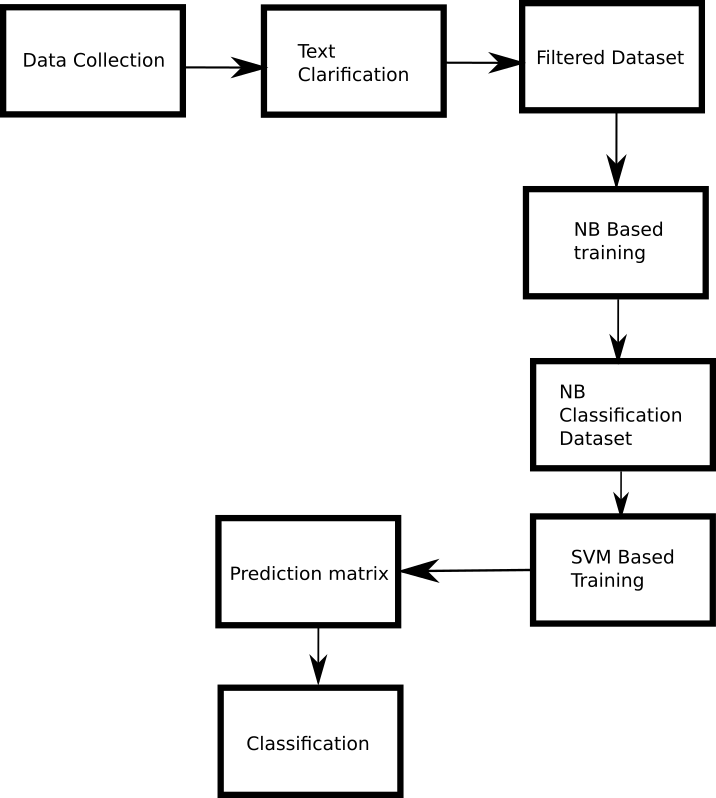
\includegraphics[width=13cm]{img/hybrid.png}
    \caption{NB-SVM Architecture (\cite{hybrid_2018})}
    \label{fig:hybrid_img}
\end{figure}